% Created by tikzDevice version 0.12.3.1 on 2023-06-16 22:25:32
% !TEX encoding = UTF-8 Unicode
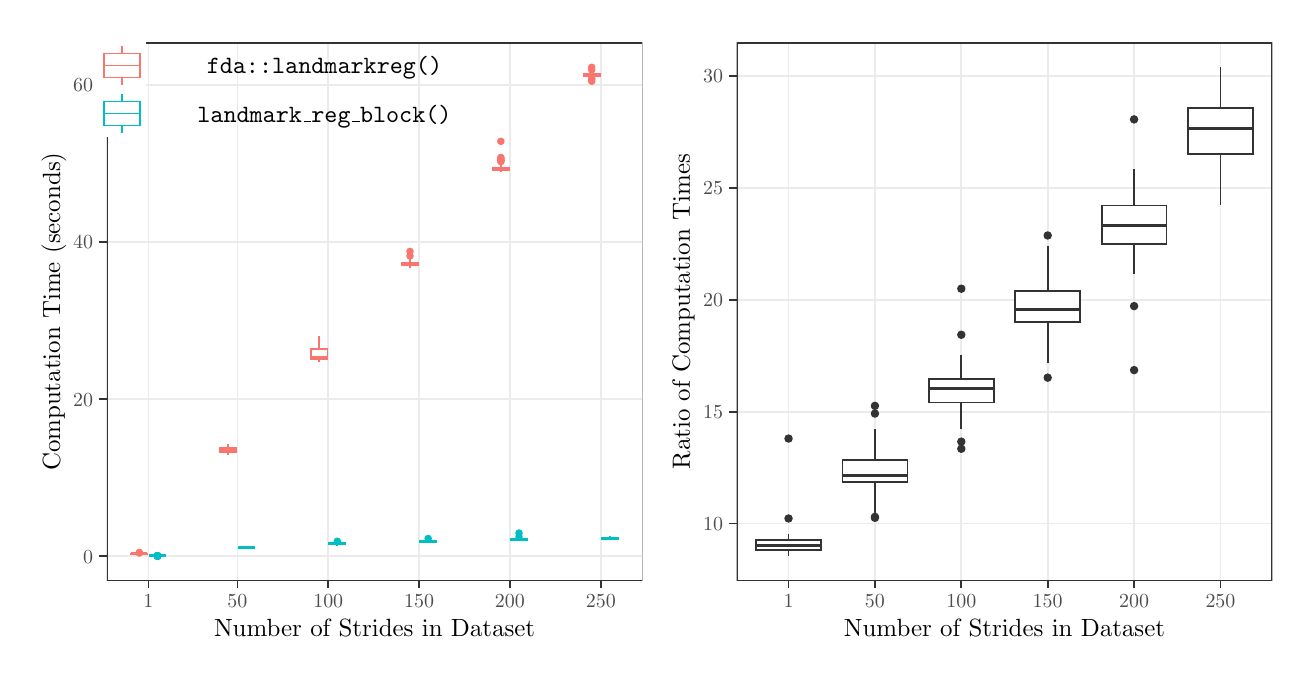
\begin{tikzpicture}[x=1pt,y=1pt]
\definecolor{fillColor}{RGB}{255,255,255}
\path[use as bounding box,fill=fillColor,fill opacity=0.00] (0,0) rectangle (455.24,227.62);
\begin{scope}
\path[clip] (  0.00,  0.00) rectangle (227.62,227.62);
\definecolor{drawColor}{RGB}{255,255,255}
\definecolor{fillColor}{RGB}{255,255,255}

\path[draw=drawColor,line width= 0.6pt,line join=round,line cap=round,fill=fillColor] ( -0.00,  0.00) rectangle (227.62,227.62);
\end{scope}
\begin{scope}
\path[clip] ( 28.58, 27.89) rectangle (222.12,222.12);
\definecolor{fillColor}{RGB}{255,255,255}

\path[fill=fillColor] ( 28.58, 27.89) rectangle (222.12,222.12);
\definecolor{drawColor}{gray}{0.92}

\path[draw=drawColor,line width= 0.6pt,line join=round] ( 28.58, 36.62) --
	(222.12, 36.62);

\path[draw=drawColor,line width= 0.6pt,line join=round] ( 28.58, 93.39) --
	(222.12, 93.39);

\path[draw=drawColor,line width= 0.6pt,line join=round] ( 28.58,150.17) --
	(222.12,150.17);

\path[draw=drawColor,line width= 0.6pt,line join=round] ( 28.58,206.94) --
	(222.12,206.94);

\path[draw=drawColor,line width= 0.6pt,line join=round] ( 43.62, 27.89) --
	( 43.62,222.12);

\path[draw=drawColor,line width= 0.6pt,line join=round] ( 75.79, 27.89) --
	( 75.79,222.12);

\path[draw=drawColor,line width= 0.6pt,line join=round] (108.61, 27.89) --
	(108.61,222.12);

\path[draw=drawColor,line width= 0.6pt,line join=round] (141.44, 27.89) --
	(141.44,222.12);

\path[draw=drawColor,line width= 0.6pt,line join=round] (174.26, 27.89) --
	(174.26,222.12);

\path[draw=drawColor,line width= 0.6pt,line join=round] (207.09, 27.89) --
	(207.09,222.12);
\definecolor{drawColor}{RGB}{248,118,109}
\definecolor{fillColor}{RGB}{248,118,109}

\path[draw=drawColor,line width= 0.4pt,line join=round,line cap=round,fill=fillColor] ( 40.34, 37.80) circle (  1.16);

\path[draw=drawColor,line width= 0.4pt,line join=round,line cap=round,fill=fillColor] ( 40.34, 37.99) circle (  1.16);

\path[draw=drawColor,line width= 0.6pt,line join=round] ( 40.34, 37.57) -- ( 40.34, 37.64);

\path[draw=drawColor,line width= 0.6pt,line join=round] ( 40.34, 37.52) -- ( 40.34, 37.51);
\definecolor{fillColor}{RGB}{255,255,255}

\path[draw=drawColor,line width= 0.6pt,fill=fillColor] ( 37.38, 37.57) --
	( 37.38, 37.52) --
	( 43.29, 37.52) --
	( 43.29, 37.57) --
	( 37.38, 37.57) --
	cycle;

\path[draw=drawColor,line width= 1.1pt] ( 37.38, 37.55) -- ( 43.29, 37.55);

\path[draw=drawColor,line width= 0.6pt,line join=round] ( 72.50, 75.67) -- ( 72.50, 77.03);

\path[draw=drawColor,line width= 0.6pt,line join=round] ( 72.50, 74.40) -- ( 72.50, 73.03);

\path[draw=drawColor,line width= 0.6pt,fill=fillColor] ( 69.55, 75.67) --
	( 69.55, 74.40) --
	( 75.46, 74.40) --
	( 75.46, 75.67) --
	( 69.55, 75.67) --
	cycle;

\path[draw=drawColor,line width= 1.1pt] ( 69.55, 74.96) -- ( 75.46, 74.96);

\path[draw=drawColor,line width= 0.6pt,line join=round] (105.33,111.49) -- (105.33,116.34);

\path[draw=drawColor,line width= 0.6pt,line join=round] (105.33,107.66) -- (105.33,106.73);

\path[draw=drawColor,line width= 0.6pt,fill=fillColor] (102.38,111.49) --
	(102.38,107.66) --
	(108.28,107.66) --
	(108.28,111.49) --
	(102.38,111.49) --
	cycle;

\path[draw=drawColor,line width= 1.1pt] (102.38,108.28) -- (108.28,108.28);
\definecolor{fillColor}{RGB}{248,118,109}

\path[draw=drawColor,line width= 0.4pt,line join=round,line cap=round,fill=fillColor] (138.15,145.14) circle (  1.16);

\path[draw=drawColor,line width= 0.4pt,line join=round,line cap=round,fill=fillColor] (138.15,146.75) circle (  1.16);

\path[draw=drawColor,line width= 0.6pt,line join=round] (138.15,142.80) -- (138.15,144.34);

\path[draw=drawColor,line width= 0.6pt,line join=round] (138.15,141.65) -- (138.15,140.61);
\definecolor{fillColor}{RGB}{255,255,255}

\path[draw=drawColor,line width= 0.6pt,fill=fillColor] (135.20,142.80) --
	(135.20,141.65) --
	(141.11,141.65) --
	(141.11,142.80) --
	(135.20,142.80) --
	cycle;

\path[draw=drawColor,line width= 1.1pt] (135.20,142.12) -- (141.11,142.12);
\definecolor{fillColor}{RGB}{248,118,109}

\path[draw=drawColor,line width= 0.4pt,line join=round,line cap=round,fill=fillColor] (170.98,186.55) circle (  1.16);

\path[draw=drawColor,line width= 0.4pt,line join=round,line cap=round,fill=fillColor] (170.98,179.65) circle (  1.16);

\path[draw=drawColor,line width= 0.4pt,line join=round,line cap=round,fill=fillColor] (170.98,180.55) circle (  1.16);

\path[draw=drawColor,line width= 0.4pt,line join=round,line cap=round,fill=fillColor] (170.98,179.26) circle (  1.16);

\path[draw=drawColor,line width= 0.4pt,line join=round,line cap=round,fill=fillColor] (170.98,179.36) circle (  1.16);

\path[draw=drawColor,line width= 0.4pt,line join=round,line cap=round,fill=fillColor] (170.98,180.00) circle (  1.16);

\path[draw=drawColor,line width= 0.4pt,line join=round,line cap=round,fill=fillColor] (170.98,180.70) circle (  1.16);

\path[draw=drawColor,line width= 0.6pt,line join=round] (170.98,177.14) -- (170.98,178.42);

\path[draw=drawColor,line width= 0.6pt,line join=round] (170.98,176.10) -- (170.98,175.54);
\definecolor{fillColor}{RGB}{255,255,255}

\path[draw=drawColor,line width= 0.6pt,fill=fillColor] (168.03,177.14) --
	(168.03,176.10) --
	(173.93,176.10) --
	(173.93,177.14) --
	(168.03,177.14) --
	cycle;

\path[draw=drawColor,line width= 1.1pt] (168.03,176.58) -- (173.93,176.58);
\definecolor{fillColor}{RGB}{248,118,109}

\path[draw=drawColor,line width= 0.4pt,line join=round,line cap=round,fill=fillColor] (203.81,213.29) circle (  1.16);

\path[draw=drawColor,line width= 0.4pt,line join=round,line cap=round,fill=fillColor] (203.81,212.41) circle (  1.16);

\path[draw=drawColor,line width= 0.4pt,line join=round,line cap=round,fill=fillColor] (203.81,209.06) circle (  1.16);

\path[draw=drawColor,line width= 0.4pt,line join=round,line cap=round,fill=fillColor] (203.81,208.27) circle (  1.16);

\path[draw=drawColor,line width= 0.4pt,line join=round,line cap=round,fill=fillColor] (203.81,209.13) circle (  1.16);

\path[draw=drawColor,line width= 0.6pt,line join=round] (203.81,210.90) -- (203.81,211.56);

\path[draw=drawColor,line width= 0.6pt,line join=round] (203.81,210.22) -- (203.81,209.33);
\definecolor{fillColor}{RGB}{255,255,255}

\path[draw=drawColor,line width= 0.6pt,fill=fillColor] (200.85,210.90) --
	(200.85,210.22) --
	(206.76,210.22) --
	(206.76,210.90) --
	(200.85,210.90) --
	cycle;

\path[draw=drawColor,line width= 1.1pt] (200.85,210.63) -- (206.76,210.63);
\definecolor{drawColor}{RGB}{0,191,196}
\definecolor{fillColor}{RGB}{0,191,196}

\path[draw=drawColor,line width= 0.4pt,line join=round,line cap=round,fill=fillColor] ( 46.90, 36.74) circle (  1.16);

\path[draw=drawColor,line width= 0.4pt,line join=round,line cap=round,fill=fillColor] ( 46.90, 36.72) circle (  1.16);

\path[draw=drawColor,line width= 0.4pt,line join=round,line cap=round,fill=fillColor] ( 46.90, 36.72) circle (  1.16);

\path[draw=drawColor,line width= 0.4pt,line join=round,line cap=round,fill=fillColor] ( 46.90, 36.72) circle (  1.16);

\path[draw=drawColor,line width= 0.4pt,line join=round,line cap=round,fill=fillColor] ( 46.90, 36.72) circle (  1.16);

\path[draw=drawColor,line width= 0.4pt,line join=round,line cap=round,fill=fillColor] ( 46.90, 36.72) circle (  1.16);

\path[draw=drawColor,line width= 0.4pt,line join=round,line cap=round,fill=fillColor] ( 46.90, 36.72) circle (  1.16);

\path[draw=drawColor,line width= 0.4pt,line join=round,line cap=round,fill=fillColor] ( 46.90, 36.72) circle (  1.16);

\path[draw=drawColor,line width= 0.4pt,line join=round,line cap=round,fill=fillColor] ( 46.90, 36.72) circle (  1.16);

\path[draw=drawColor,line width= 0.4pt,line join=round,line cap=round,fill=fillColor] ( 46.90, 36.72) circle (  1.16);

\path[draw=drawColor,line width= 0.4pt,line join=round,line cap=round,fill=fillColor] ( 46.90, 36.72) circle (  1.16);

\path[draw=drawColor,line width= 0.4pt,line join=round,line cap=round,fill=fillColor] ( 46.90, 36.72) circle (  1.16);

\path[draw=drawColor,line width= 0.4pt,line join=round,line cap=round,fill=fillColor] ( 46.90, 36.72) circle (  1.16);

\path[draw=drawColor,line width= 0.4pt,line join=round,line cap=round,fill=fillColor] ( 46.90, 36.72) circle (  1.16);

\path[draw=drawColor,line width= 0.4pt,line join=round,line cap=round,fill=fillColor] ( 46.90, 36.72) circle (  1.16);

\path[draw=drawColor,line width= 0.4pt,line join=round,line cap=round,fill=fillColor] ( 46.90, 36.73) circle (  1.16);

\path[draw=drawColor,line width= 0.4pt,line join=round,line cap=round,fill=fillColor] ( 46.90, 36.73) circle (  1.16);

\path[draw=drawColor,line width= 0.4pt,line join=round,line cap=round,fill=fillColor] ( 46.90, 36.72) circle (  1.16);

\path[draw=drawColor,line width= 0.4pt,line join=round,line cap=round,fill=fillColor] ( 46.90, 36.72) circle (  1.16);

\path[draw=drawColor,line width= 0.4pt,line join=round,line cap=round,fill=fillColor] ( 46.90, 36.73) circle (  1.16);

\path[draw=drawColor,line width= 0.4pt,line join=round,line cap=round,fill=fillColor] ( 46.90, 36.72) circle (  1.16);

\path[draw=drawColor,line width= 0.6pt,line join=round] ( 46.90, 36.72) -- ( 46.90, 36.72);

\path[draw=drawColor,line width= 0.6pt,line join=round] ( 46.90, 36.72) -- ( 46.90, 36.72);
\definecolor{fillColor}{RGB}{255,255,255}

\path[draw=drawColor,line width= 0.6pt,fill=fillColor] ( 43.95, 36.72) --
	( 43.95, 36.72) --
	( 49.85, 36.72) --
	( 49.85, 36.72) --
	( 43.95, 36.72) --
	cycle;

\path[draw=drawColor,line width= 1.1pt] ( 43.95, 36.72) -- ( 49.85, 36.72);

\path[draw=drawColor,line width= 0.6pt,line join=round] ( 79.07, 39.94) -- ( 79.07, 40.41);

\path[draw=drawColor,line width= 0.6pt,line join=round] ( 79.07, 39.58) -- ( 79.07, 39.11);

\path[draw=drawColor,line width= 0.6pt,fill=fillColor] ( 76.12, 39.94) --
	( 76.12, 39.58) --
	( 82.02, 39.58) --
	( 82.02, 39.94) --
	( 76.12, 39.94) --
	cycle;

\path[draw=drawColor,line width= 1.1pt] ( 76.12, 39.78) -- ( 82.02, 39.78);
\definecolor{fillColor}{RGB}{0,191,196}

\path[draw=drawColor,line width= 0.4pt,line join=round,line cap=round,fill=fillColor] (111.89, 42.02) circle (  1.16);

\path[draw=drawColor,line width= 0.6pt,line join=round] (111.89, 41.38) -- (111.89, 41.92);

\path[draw=drawColor,line width= 0.6pt,line join=round] (111.89, 40.96) -- (111.89, 40.41);
\definecolor{fillColor}{RGB}{255,255,255}

\path[draw=drawColor,line width= 0.6pt,fill=fillColor] (108.94, 41.38) --
	(108.94, 40.96) --
	(114.85, 40.96) --
	(114.85, 41.38) --
	(108.94, 41.38) --
	cycle;

\path[draw=drawColor,line width= 1.1pt] (108.94, 41.15) -- (114.85, 41.15);
\definecolor{fillColor}{RGB}{0,191,196}

\path[draw=drawColor,line width= 0.4pt,line join=round,line cap=round,fill=fillColor] (144.72, 43.02) circle (  1.16);

\path[draw=drawColor,line width= 0.6pt,line join=round] (144.72, 42.18) -- (144.72, 42.71);

\path[draw=drawColor,line width= 0.6pt,line join=round] (144.72, 41.78) -- (144.72, 41.26);
\definecolor{fillColor}{RGB}{255,255,255}

\path[draw=drawColor,line width= 0.6pt,fill=fillColor] (141.77, 42.18) --
	(141.77, 41.78) --
	(147.67, 41.78) --
	(147.67, 42.18) --
	(141.77, 42.18) --
	cycle;

\path[draw=drawColor,line width= 1.1pt] (141.77, 42.03) -- (147.67, 42.03);
\definecolor{fillColor}{RGB}{0,191,196}

\path[draw=drawColor,line width= 0.4pt,line join=round,line cap=round,fill=fillColor] (177.54, 43.73) circle (  1.16);

\path[draw=drawColor,line width= 0.4pt,line join=round,line cap=round,fill=fillColor] (177.54, 45.01) circle (  1.16);

\path[draw=drawColor,line width= 0.6pt,line join=round] (177.54, 42.83) -- (177.54, 43.20);

\path[draw=drawColor,line width= 0.6pt,line join=round] (177.54, 42.42) -- (177.54, 41.96);
\definecolor{fillColor}{RGB}{255,255,255}

\path[draw=drawColor,line width= 0.6pt,fill=fillColor] (174.59, 42.83) --
	(174.59, 42.42) --
	(180.50, 42.42) --
	(180.50, 42.83) --
	(174.59, 42.83) --
	cycle;

\path[draw=drawColor,line width= 1.1pt] (174.59, 42.60) -- (180.50, 42.60);

\path[draw=drawColor,line width= 0.6pt,line join=round] (210.37, 43.19) -- (210.37, 43.77);

\path[draw=drawColor,line width= 0.6pt,line join=round] (210.37, 42.70) -- (210.37, 42.37);

\path[draw=drawColor,line width= 0.6pt,fill=fillColor] (207.42, 43.19) --
	(207.42, 42.70) --
	(213.32, 42.70) --
	(213.32, 43.19) --
	(207.42, 43.19) --
	cycle;

\path[draw=drawColor,line width= 1.1pt] (207.42, 42.92) -- (213.32, 42.92);
\definecolor{drawColor}{gray}{0.20}

\path[draw=drawColor,line width= 0.6pt,line join=round,line cap=round] ( 28.58, 27.89) rectangle (222.12,222.12);
\end{scope}
\begin{scope}
\path[clip] (  0.00,  0.00) rectangle (455.24,227.62);
\definecolor{drawColor}{gray}{0.30}

\node[text=drawColor,anchor=base east,inner sep=0pt, outer sep=0pt, scale=  0.72] at ( 23.63, 34.14) {0};

\node[text=drawColor,anchor=base east,inner sep=0pt, outer sep=0pt, scale=  0.72] at ( 23.63, 90.91) {20};

\node[text=drawColor,anchor=base east,inner sep=0pt, outer sep=0pt, scale=  0.72] at ( 23.63,147.69) {40};

\node[text=drawColor,anchor=base east,inner sep=0pt, outer sep=0pt, scale=  0.72] at ( 23.63,204.46) {60};
\end{scope}
\begin{scope}
\path[clip] (  0.00,  0.00) rectangle (455.24,227.62);
\definecolor{drawColor}{gray}{0.20}

\path[draw=drawColor,line width= 0.6pt,line join=round] ( 25.83, 36.62) --
	( 28.58, 36.62);

\path[draw=drawColor,line width= 0.6pt,line join=round] ( 25.83, 93.39) --
	( 28.58, 93.39);

\path[draw=drawColor,line width= 0.6pt,line join=round] ( 25.83,150.17) --
	( 28.58,150.17);

\path[draw=drawColor,line width= 0.6pt,line join=round] ( 25.83,206.94) --
	( 28.58,206.94);
\end{scope}
\begin{scope}
\path[clip] (  0.00,  0.00) rectangle (455.24,227.62);
\definecolor{drawColor}{gray}{0.20}

\path[draw=drawColor,line width= 0.6pt,line join=round] ( 43.62, 25.14) --
	( 43.62, 27.89);

\path[draw=drawColor,line width= 0.6pt,line join=round] ( 75.79, 25.14) --
	( 75.79, 27.89);

\path[draw=drawColor,line width= 0.6pt,line join=round] (108.61, 25.14) --
	(108.61, 27.89);

\path[draw=drawColor,line width= 0.6pt,line join=round] (141.44, 25.14) --
	(141.44, 27.89);

\path[draw=drawColor,line width= 0.6pt,line join=round] (174.26, 25.14) --
	(174.26, 27.89);

\path[draw=drawColor,line width= 0.6pt,line join=round] (207.09, 25.14) --
	(207.09, 27.89);
\end{scope}
\begin{scope}
\path[clip] (  0.00,  0.00) rectangle (455.24,227.62);
\definecolor{drawColor}{gray}{0.30}

\node[text=drawColor,anchor=base,inner sep=0pt, outer sep=0pt, scale=  0.72] at ( 43.62, 17.98) {1};

\node[text=drawColor,anchor=base,inner sep=0pt, outer sep=0pt, scale=  0.72] at ( 75.79, 17.98) {50};

\node[text=drawColor,anchor=base,inner sep=0pt, outer sep=0pt, scale=  0.72] at (108.61, 17.98) {100};

\node[text=drawColor,anchor=base,inner sep=0pt, outer sep=0pt, scale=  0.72] at (141.44, 17.98) {150};

\node[text=drawColor,anchor=base,inner sep=0pt, outer sep=0pt, scale=  0.72] at (174.26, 17.98) {200};

\node[text=drawColor,anchor=base,inner sep=0pt, outer sep=0pt, scale=  0.72] at (207.09, 17.98) {250};
\end{scope}
\begin{scope}
\path[clip] (  0.00,  0.00) rectangle (455.24,227.62);
\definecolor{drawColor}{RGB}{0,0,0}

\node[text=drawColor,anchor=base,inner sep=0pt, outer sep=0pt, scale=  0.90] at (125.35,  7.49) {Number of Strides in Dataset};
\end{scope}
\begin{scope}
\path[clip] (  0.00,  0.00) rectangle (455.24,227.62);
\definecolor{drawColor}{RGB}{0,0,0}

\node[text=drawColor,rotate= 90.00,anchor=base,inner sep=0pt, outer sep=0pt, scale=  0.90] at ( 11.70,125.01) {Computation Time (seconds)};
\end{scope}
\begin{scope}
\path[clip] (  0.00,  0.00) rectangle (455.24,227.62);
\definecolor{fillColor}{RGB}{255,255,255}

\path[fill=fillColor] ( 25.31,205.30) rectangle ( 42.65,222.65);
\end{scope}
\begin{scope}
\path[clip] (  0.00,  0.00) rectangle (455.24,227.62);
\definecolor{drawColor}{RGB}{248,118,109}

\path[draw=drawColor,line width= 0.6pt] ( 33.98,207.04) --
	( 33.98,209.64);

\path[draw=drawColor,line width= 0.6pt] ( 33.98,218.31) --
	( 33.98,220.91);
\definecolor{fillColor}{RGB}{255,255,255}

\path[draw=drawColor,line width= 0.6pt,fill=fillColor] ( 27.48,209.64) rectangle ( 40.48,218.31);

\path[draw=drawColor,line width= 0.6pt] ( 27.48,213.98) --
	( 40.48,213.98);
\end{scope}
\begin{scope}
\path[clip] (  0.00,  0.00) rectangle (455.24,227.62);
\definecolor{fillColor}{RGB}{255,255,255}

\path[fill=fillColor] ( 25.31,187.96) rectangle ( 42.65,205.30);
\end{scope}
\begin{scope}
\path[clip] (  0.00,  0.00) rectangle (455.24,227.62);
\definecolor{drawColor}{RGB}{0,191,196}

\path[draw=drawColor,line width= 0.6pt] ( 33.98,189.69) --
	( 33.98,192.30);

\path[draw=drawColor,line width= 0.6pt] ( 33.98,200.97) --
	( 33.98,203.57);
\definecolor{fillColor}{RGB}{255,255,255}

\path[draw=drawColor,line width= 0.6pt,fill=fillColor] ( 27.48,192.30) rectangle ( 40.48,200.97);

\path[draw=drawColor,line width= 0.6pt] ( 27.48,196.63) --
	( 40.48,196.63);
\end{scope}
\begin{scope}
\path[clip] (  0.00,  0.00) rectangle (455.24,227.62);
\definecolor{drawColor}{RGB}{0,0,0}

\node[text=drawColor,anchor=base,inner sep=0pt, outer sep=0pt, scale=  0.90] at (107.24,210.88) {\texttt{fda::landmarkreg()}};
\end{scope}
\begin{scope}
\path[clip] (  0.00,  0.00) rectangle (455.24,227.62);
\definecolor{drawColor}{RGB}{0,0,0}

\node[text=drawColor,anchor=base,inner sep=0pt, outer sep=0pt, scale=  0.90] at (107.24,193.53) {\texttt{landmark\_reg\_block()}};
\end{scope}
\begin{scope}
\path[clip] (227.62,  0.00) rectangle (455.24,227.62);
\definecolor{drawColor}{RGB}{255,255,255}
\definecolor{fillColor}{RGB}{255,255,255}

\path[draw=drawColor,line width= 0.6pt,line join=round,line cap=round,fill=fillColor] (227.62,  0.00) rectangle (455.24,227.62);
\end{scope}
\begin{scope}
\path[clip] (256.21, 27.89) rectangle (449.74,222.12);
\definecolor{fillColor}{RGB}{255,255,255}

\path[fill=fillColor] (256.21, 27.89) rectangle (449.74,222.12);
\definecolor{drawColor}{gray}{0.92}

\path[draw=drawColor,line width= 0.6pt,line join=round] (256.21, 48.42) --
	(449.74, 48.42);

\path[draw=drawColor,line width= 0.6pt,line join=round] (256.21, 88.85) --
	(449.74, 88.85);

\path[draw=drawColor,line width= 0.6pt,line join=round] (256.21,129.27) --
	(449.74,129.27);

\path[draw=drawColor,line width= 0.6pt,line join=round] (256.21,169.70) --
	(449.74,169.70);

\path[draw=drawColor,line width= 0.6pt,line join=round] (256.21,210.12) --
	(449.74,210.12);

\path[draw=drawColor,line width= 0.6pt,line join=round] (274.94, 27.89) --
	(274.94,222.12);

\path[draw=drawColor,line width= 0.6pt,line join=round] (306.15, 27.89) --
	(306.15,222.12);

\path[draw=drawColor,line width= 0.6pt,line join=round] (337.37, 27.89) --
	(337.37,222.12);

\path[draw=drawColor,line width= 0.6pt,line join=round] (368.58, 27.89) --
	(368.58,222.12);

\path[draw=drawColor,line width= 0.6pt,line join=round] (399.80, 27.89) --
	(399.80,222.12);

\path[draw=drawColor,line width= 0.6pt,line join=round] (431.01, 27.89) --
	(431.01,222.12);
\definecolor{drawColor}{gray}{0.20}
\definecolor{fillColor}{gray}{0.20}

\path[draw=drawColor,line width= 0.4pt,line join=round,line cap=round,fill=fillColor] (274.94, 79.14) circle (  1.32);

\path[draw=drawColor,line width= 0.4pt,line join=round,line cap=round,fill=fillColor] (274.94, 50.27) circle (  1.32);

\path[draw=drawColor,line width= 0.6pt,line join=round] (274.94, 42.58) -- (274.94, 44.83);

\path[draw=drawColor,line width= 0.6pt,line join=round] (274.94, 38.76) -- (274.94, 36.72);
\definecolor{fillColor}{RGB}{255,255,255}

\path[draw=drawColor,line width= 0.6pt,fill=fillColor] (263.23, 42.58) --
	(263.23, 38.76) --
	(286.64, 38.76) --
	(286.64, 42.58) --
	(263.23, 42.58) --
	cycle;

\path[draw=drawColor,line width= 1.1pt] (263.23, 40.45) -- (286.64, 40.45);
\definecolor{fillColor}{gray}{0.20}

\path[draw=drawColor,line width= 0.4pt,line join=round,line cap=round,fill=fillColor] (306.15, 90.96) circle (  1.32);

\path[draw=drawColor,line width= 0.4pt,line join=round,line cap=round,fill=fillColor] (306.15, 88.18) circle (  1.32);

\path[draw=drawColor,line width= 0.4pt,line join=round,line cap=round,fill=fillColor] (306.15, 50.50) circle (  1.32);

\path[draw=drawColor,line width= 0.4pt,line join=round,line cap=round,fill=fillColor] (306.15, 50.85) circle (  1.32);

\path[draw=drawColor,line width= 0.6pt,line join=round] (306.15, 71.39) -- (306.15, 82.52);

\path[draw=drawColor,line width= 0.6pt,line join=round] (306.15, 63.49) -- (306.15, 52.42);
\definecolor{fillColor}{RGB}{255,255,255}

\path[draw=drawColor,line width= 0.6pt,fill=fillColor] (294.44, 71.39) --
	(294.44, 63.49) --
	(317.86, 63.49) --
	(317.86, 71.39) --
	(294.44, 71.39) --
	cycle;

\path[draw=drawColor,line width= 1.1pt] (294.44, 65.96) -- (317.86, 65.96);
\definecolor{fillColor}{gray}{0.20}

\path[draw=drawColor,line width= 0.4pt,line join=round,line cap=round,fill=fillColor] (337.37,133.30) circle (  1.32);

\path[draw=drawColor,line width= 0.4pt,line join=round,line cap=round,fill=fillColor] (337.37,116.65) circle (  1.32);

\path[draw=drawColor,line width= 0.4pt,line join=round,line cap=round,fill=fillColor] (337.37, 75.46) circle (  1.32);

\path[draw=drawColor,line width= 0.4pt,line join=round,line cap=round,fill=fillColor] (337.37, 78.03) circle (  1.32);

\path[draw=drawColor,line width= 0.6pt,line join=round] (337.37,100.72) -- (337.37,109.26);

\path[draw=drawColor,line width= 0.6pt,line join=round] (337.37, 92.18) -- (337.37, 82.63);
\definecolor{fillColor}{RGB}{255,255,255}

\path[draw=drawColor,line width= 0.6pt,fill=fillColor] (325.66,100.72) --
	(325.66, 92.18) --
	(349.07, 92.18) --
	(349.07,100.72) --
	(325.66,100.72) --
	cycle;

\path[draw=drawColor,line width= 1.1pt] (325.66, 97.32) -- (349.07, 97.32);
\definecolor{fillColor}{gray}{0.20}

\path[draw=drawColor,line width= 0.4pt,line join=round,line cap=round,fill=fillColor] (368.58,152.53) circle (  1.32);

\path[draw=drawColor,line width= 0.4pt,line join=round,line cap=round,fill=fillColor] (368.58,101.15) circle (  1.32);

\path[draw=drawColor,line width= 0.6pt,line join=round] (368.58,132.53) -- (368.58,148.71);

\path[draw=drawColor,line width= 0.6pt,line join=round] (368.58,121.24) -- (368.58,106.39);
\definecolor{fillColor}{RGB}{255,255,255}

\path[draw=drawColor,line width= 0.6pt,fill=fillColor] (356.88,132.53) --
	(356.88,121.24) --
	(380.29,121.24) --
	(380.29,132.53) --
	(356.88,132.53) --
	cycle;

\path[draw=drawColor,line width= 1.1pt] (356.88,125.61) -- (380.29,125.61);
\definecolor{fillColor}{gray}{0.20}

\path[draw=drawColor,line width= 0.4pt,line join=round,line cap=round,fill=fillColor] (399.80,194.47) circle (  1.32);

\path[draw=drawColor,line width= 0.4pt,line join=round,line cap=round,fill=fillColor] (399.80,127.01) circle (  1.32);

\path[draw=drawColor,line width= 0.4pt,line join=round,line cap=round,fill=fillColor] (399.80,103.88) circle (  1.32);

\path[draw=drawColor,line width= 0.6pt,line join=round] (399.80,163.31) -- (399.80,176.50);

\path[draw=drawColor,line width= 0.6pt,line join=round] (399.80,149.34) -- (399.80,138.66);
\definecolor{fillColor}{RGB}{255,255,255}

\path[draw=drawColor,line width= 0.6pt,fill=fillColor] (388.09,163.31) --
	(388.09,149.34) --
	(411.50,149.34) --
	(411.50,163.31) --
	(388.09,163.31) --
	cycle;

\path[draw=drawColor,line width= 1.1pt] (388.09,156.10) -- (411.50,156.10);

\path[draw=drawColor,line width= 0.6pt,line join=round] (431.01,198.65) -- (431.01,213.29);

\path[draw=drawColor,line width= 0.6pt,line join=round] (431.01,182.02) -- (431.01,163.70);

\path[draw=drawColor,line width= 0.6pt,fill=fillColor] (419.31,198.65) --
	(419.31,182.02) --
	(442.72,182.02) --
	(442.72,198.65) --
	(419.31,198.65) --
	cycle;

\path[draw=drawColor,line width= 1.1pt] (419.31,191.12) -- (442.72,191.12);

\path[draw=drawColor,line width= 0.6pt,line join=round,line cap=round] (256.21, 27.89) rectangle (449.74,222.12);
\end{scope}
\begin{scope}
\path[clip] (  0.00,  0.00) rectangle (455.24,227.62);
\definecolor{drawColor}{gray}{0.30}

\node[text=drawColor,anchor=base east,inner sep=0pt, outer sep=0pt, scale=  0.72] at (251.26, 45.94) {10};

\node[text=drawColor,anchor=base east,inner sep=0pt, outer sep=0pt, scale=  0.72] at (251.26, 86.37) {15};

\node[text=drawColor,anchor=base east,inner sep=0pt, outer sep=0pt, scale=  0.72] at (251.26,126.79) {20};

\node[text=drawColor,anchor=base east,inner sep=0pt, outer sep=0pt, scale=  0.72] at (251.26,167.22) {25};

\node[text=drawColor,anchor=base east,inner sep=0pt, outer sep=0pt, scale=  0.72] at (251.26,207.64) {30};
\end{scope}
\begin{scope}
\path[clip] (  0.00,  0.00) rectangle (455.24,227.62);
\definecolor{drawColor}{gray}{0.20}

\path[draw=drawColor,line width= 0.6pt,line join=round] (253.46, 48.42) --
	(256.21, 48.42);

\path[draw=drawColor,line width= 0.6pt,line join=round] (253.46, 88.85) --
	(256.21, 88.85);

\path[draw=drawColor,line width= 0.6pt,line join=round] (253.46,129.27) --
	(256.21,129.27);

\path[draw=drawColor,line width= 0.6pt,line join=round] (253.46,169.70) --
	(256.21,169.70);

\path[draw=drawColor,line width= 0.6pt,line join=round] (253.46,210.12) --
	(256.21,210.12);
\end{scope}
\begin{scope}
\path[clip] (  0.00,  0.00) rectangle (455.24,227.62);
\definecolor{drawColor}{gray}{0.20}

\path[draw=drawColor,line width= 0.6pt,line join=round] (274.94, 25.14) --
	(274.94, 27.89);

\path[draw=drawColor,line width= 0.6pt,line join=round] (306.15, 25.14) --
	(306.15, 27.89);

\path[draw=drawColor,line width= 0.6pt,line join=round] (337.37, 25.14) --
	(337.37, 27.89);

\path[draw=drawColor,line width= 0.6pt,line join=round] (368.58, 25.14) --
	(368.58, 27.89);

\path[draw=drawColor,line width= 0.6pt,line join=round] (399.80, 25.14) --
	(399.80, 27.89);

\path[draw=drawColor,line width= 0.6pt,line join=round] (431.01, 25.14) --
	(431.01, 27.89);
\end{scope}
\begin{scope}
\path[clip] (  0.00,  0.00) rectangle (455.24,227.62);
\definecolor{drawColor}{gray}{0.30}

\node[text=drawColor,anchor=base,inner sep=0pt, outer sep=0pt, scale=  0.72] at (274.94, 17.98) {1};

\node[text=drawColor,anchor=base,inner sep=0pt, outer sep=0pt, scale=  0.72] at (306.15, 17.98) {50};

\node[text=drawColor,anchor=base,inner sep=0pt, outer sep=0pt, scale=  0.72] at (337.37, 17.98) {100};

\node[text=drawColor,anchor=base,inner sep=0pt, outer sep=0pt, scale=  0.72] at (368.58, 17.98) {150};

\node[text=drawColor,anchor=base,inner sep=0pt, outer sep=0pt, scale=  0.72] at (399.80, 17.98) {200};

\node[text=drawColor,anchor=base,inner sep=0pt, outer sep=0pt, scale=  0.72] at (431.01, 17.98) {250};
\end{scope}
\begin{scope}
\path[clip] (  0.00,  0.00) rectangle (455.24,227.62);
\definecolor{drawColor}{RGB}{0,0,0}

\node[text=drawColor,anchor=base,inner sep=0pt, outer sep=0pt, scale=  0.90] at (352.97,  7.49) {Number of Strides in Dataset};
\end{scope}
\begin{scope}
\path[clip] (  0.00,  0.00) rectangle (455.24,227.62);
\definecolor{drawColor}{RGB}{0,0,0}

\node[text=drawColor,rotate= 90.00,anchor=base,inner sep=0pt, outer sep=0pt, scale=  0.90] at (239.32,125.01) {Ratio of Computation Times};
\end{scope}
\end{tikzpicture}
